%%%%%%%%%%%%%%%%%%%%%%%%%%%%%%%%%%%%%%%%%
% Short Sectioned Assignment
% LaTeX Template
% Version 1.0 (5/5/12)
%
% This template has been downloaded from:
% http://www.LaTeXTemplates.com
%
% Original author:
% Frits Wenneker (http://www.howtotex.com)
%
% License:
% CC BY-NC-SA 3.0 (http://creativecommons.org/licenses/by-nc-sa/3.0/)
%
%%%%%%%%%%%%%%%%%%%%%%%%%%%%%%%%%%%%%%%%%

%----------------------------------------------------------------------------------------
%	PACKAGES AND OTHER DOCUMENT CONFIGURATIONS
%----------------------------------------------------------------------------------------

\documentclass[paper=a4, fontsize=9pt]{scrartcl} % A4 paper and 11pt font size


\usepackage[T1]{fontenc} % Use 8-bit encoding that has 256 glyphs
\usepackage[english,francais]{babel} % Français et anglais
\usepackage[utf8]{inputenc} 

\usepackage{amsmath,amsfonts,amsthm} % Math packages

\usepackage{enumitem}
\usepackage{lmodern}
\usepackage{url}
\usepackage{eurosym} % signe Euros
\usepackage{geometry} % Pour passer au format A4
\geometry{a4paper} % 
\usepackage{graphicx} % Required for including pictures
\usepackage{float} % Allows putting an [H] in \begin{figure} to specify the exact location of the figure

\usepackage{multicol}

\usepackage{verbatim}

\usepackage{sectsty} % Allows customizing section commands
\allsectionsfont{\centering \normalfont\scshape} % Make all sections centered, the default font and small caps

%----------------------------------------------------------------------------------------
%	Pied de Page
%----------------------------------------------------------------------------------------


\usepackage{fancyhdr} % Custom headers and footers
\pagestyle{fancyplain} % Makes all pages in the document conform to the custom headers and footers
\fancyhead{} % No page header - if you want one, create it in the same way as the footers below
\fancyfoot[C]{Calcul Littéral} % Empty center footer
\fancyfoot[R]{\thepage} % Page numbering for right footer

\renewcommand{\headrulewidth}{0pt} % Remove header underlines
\renewcommand{\footrulewidth}{0pt} % Remove footer underlines

%\usepackage{titling}
%\setlength{\droptitle}{-2.5cm}
%\setlength{\headheight}{13.6pt} % Customize the height of the header

\setlength\parindent{0pt} % Removes all indentation from paragraphs - comment this line for an assignment with lots of text


%----------------------------------------------------------------------------------------
%	Titre
%----------------------------------------------------------------------------------------

\newcommand{\horrule}[1]{\rule{\linewidth}{#1}} % Create horizontal rule command with 1 argument of height


\title{	
  \vspace{-14ex}
  \horrule{0.5pt} \\[0.4cm] % Thin top horizontal rule
  \huge Calcul littéral \\ % The assignment title
  \horrule{2pt} \\[0.5cm] % Thick bottom horizontal rule
}

\author{}
\date{\vspace{-10ex}} % Today's date or a custom date

%----------------------------------------------------------------------------------------
%	Début du document
%----------------------------------------------------------------------------------------

\begin{document}

%----------------------------------------------------------------------------------------
% RE-DEFINITION
%----------------------------------------------------------------------------------------
% MATHS
%-----------

\newtheorem{Definition}{Définition}
\newtheorem{Theorem}{Théorème}
\newtheorem{Proposition}{Propriété}

% MATHS
%-----------
\renewcommand{\labelitemi}{$\bullet$}
\renewcommand{\labelitemii}{$\circ$}
%----------------------------------------------------------------------------------------
%	Titre
%----------------------------------------------------------------------------------------

\maketitle % Print the title
\setlength{\columnseprule}{1pt}

\begin{Definition}
  Un calcul littéral est un calcul où l'ensemble des nombres ne sont pas connus. On représente ces \textbf{inconnus} par des \textbf{lettres}.
\end{Definition}

\begin{multicols}{2}

  \section{Programme de calcul}
  Un programme de calcul est un ensemble d'instructions et d'opérations à faire les uns à la suite des autres.

  \begin{itemize}
  \item Choisir un nombre.
  \item Multiplier par 2.
  \item Soustraire 3 au résultat.
  \item Afficher le résultat.
  \end{itemize}

\end{multicols}

\begin{enumerate}
\item[a)] Essayer avec les nombres suivants : $3$, $10$, $12$ et $-2$.
\item[b)] On prend $x$ comme nombre de départ. Exécuter le programme de calcul. 
\item[c)] Évaluer le programme avec $x=0$, $x=1$ , $x=2$ et $x=3$.
\end{enumerate}

\begin{Proposition}
Pour trouver le résultat pour une certaine valeur de $x$, on remplace tous les $x$ présents par la valeur souhaitée. On a \textbf{évalué} pour une certaine valeur de $x$.
\end{Proposition}

\horrule{1px}

\begin{multicols}{2}

\section{Règles d'écriture}

  \begin{Proposition}
    Le signe $\times$ de la multiplication n'est pas obligatoirement écrit.\\

    $2 \times x          = 2x$\\
    $3 \times (2 + x)    = 3(2 + x)$\\ 
    $v \times t          = vt$\\
    $2 \times a \times 3 = 2 \times 3 \times a = 6 \times a = 6a$\\
    \vspace{0.3cm}\\
    Le 1 devant une lettre ne doit pas être écrit. Zéro fois une lettre est égale à 0. \\
    $1 \times x          = 1x = x$ \\
    $0 \times x          = 0x = 0$
  \end{Proposition} 


  \begin{Proposition}
    On peut additionner (ou soustraire) des mêmes lettres.
    $$2x + 3x - 10x = 5x - 10x = -5x$$
    On ne peut pas additionner ou soustraire une lettre et un nombre.
    $$1 + 2x + 3 - 4x = 4 - 2x$$
    On ne peut pas additionner ou soustraire deux lettres différentes. 
    $$1 + a + 2b + 3a +4b = 1 + 4a + 6b$$
    $$1 + x + x^2 + 2 + 3x + 4x^2 = 3 + 4x + 5x^2$$
  \end{Proposition}

\end{multicols}

\horrule{1px}

\section{Distributivité}

\fbox{\parbox{\textwidth}{
    $$k (a + b) = ka + kb$$
    $$k (a - b) = ka - kb$$ 
}}

\begin{multicols}{2}
Réduire : $2(x + 3)$\\
$ 2(x + 3) = 2 \times x + 2 \times 3$ \\
$ 2(x + 3) = 2x + 6$\\

Vérifier pour $x= 4$.\\
$ 2(4 + 3) = 2 \times 7 = 14$\\
$ 2(4 + 3) = 2 \times 4 + 2 \times 3 = 8 + 6 = 14$\\

\begin{figure}[H]
  \centering
  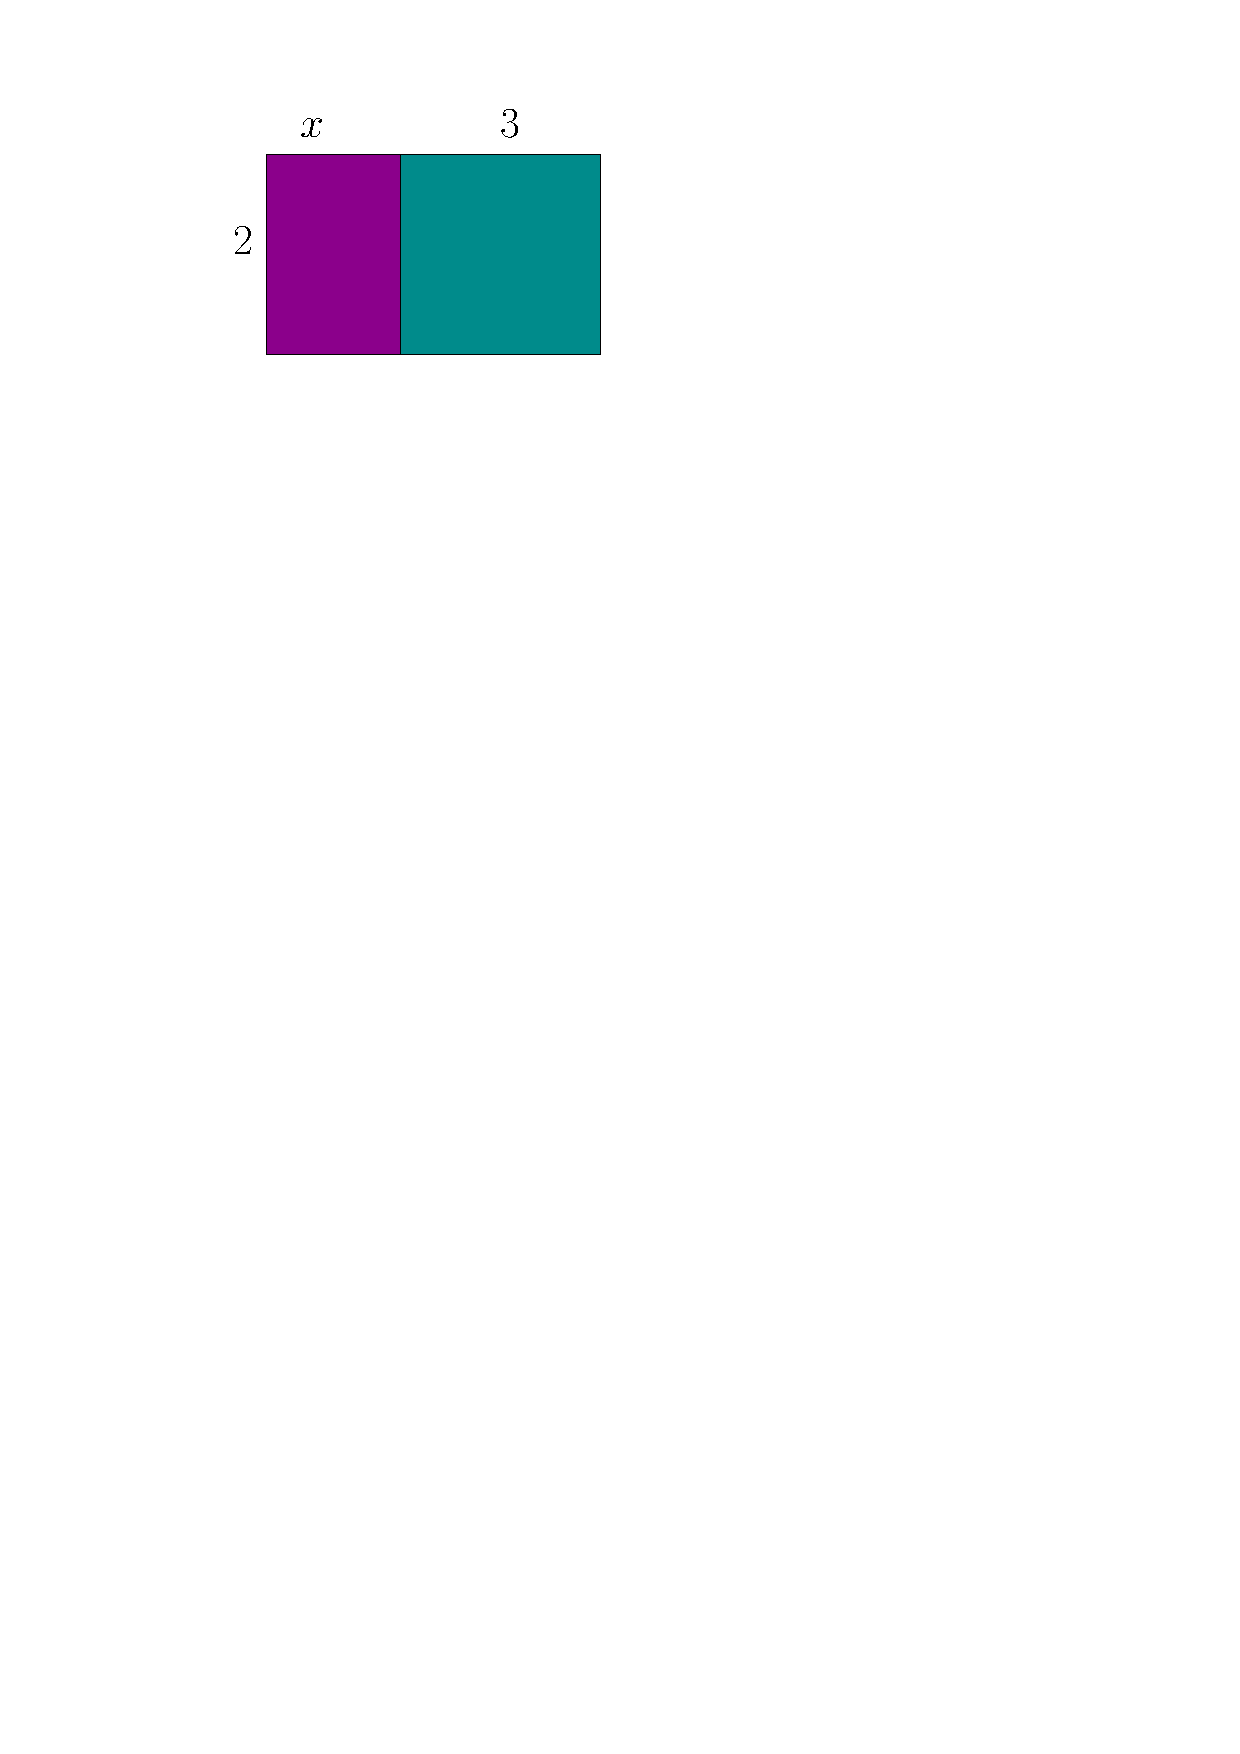
\includegraphics[width=0.8\linewidth]{sources/1/simple-distri.pdf}
\end{figure}

\end{multicols}
\end{document}
